\section{Ariel 操作系统概述 %\& User Guide
}\label{sec:user-guide}

 \begin{figure}[t!]
     \centering
     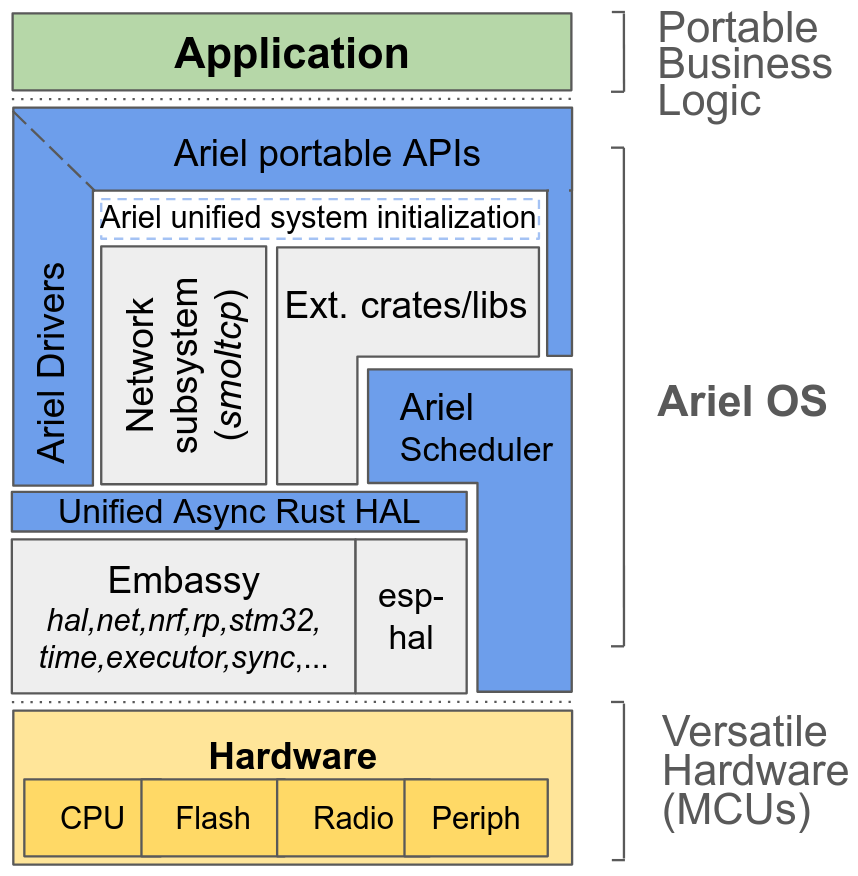
\includegraphics[width=0.7\linewidth]{translate/figures/arch-diagram-v4.png}
     \caption{\OSname{} 体系结构图%\noteCA{Ariel portable APIs also reach down to the Ariel scheduler; making it more closed and less fragmented. And this will need a color code legend.}
     }
     \label{fig:ariel-arch}
 \end{figure}
 

%\noteEB{Kaspar TO DO: choose a diagram ;)} \noteKS{I prefer EB's diagram, I tried to put in more embassy}
%Beyond its scheduler, \OSname{} aims to be a one-stop-shop for distributed computing and networked applications on heterogeneous 32-bit MCUs.
% \OSname{} is fully open-source~\cite{ariel-os-repo}. For basic hardware abstraction and async Rust programming, \OSname{} builds on top of Embassy~\cite{embassy}. Fig. \ref{fig:ariel-arch} shows how \OSname{} components (in blue) harness the ecosystem of embedded Rust (in grey).
% In particular, \OSname{} combines the following elements:
\OSname{}是完全开源的~\cite{ariel-os-repo}。对于基础硬件抽象和异步Rust编程,\OSname{}基于Embassy构建~\cite{embassy}。图\ref{fig:ariel-arch}展示了\OSname{}组件(蓝色部分)是如何利用嵌入式Rust生态系统(灰色部分)的。
具体来说,\OSname{}结合了以下元素:
%It tries to achieve that by increasing the level of abstraction, providing re-usable building blocks with usable defaults, better supporting diverse configurations in the build system, reducing boiler plate... higher level of abstraction makes high-level features possible ...
%\noteCA{… ``by providing convenient defaults for repetitive tasks of application developers''? (may be in a direction not useful for the audience, EB has opinion)}
\iffalse
\begin{itemize}
    \item Abstracting system initialization: system initialization is provided
    \item Unified peripheral APIs for application code portability: hardware access (sensor/actuator abstraction); network access (sock equivalent?). Code re-use of business logic across HW, e.g., our benchmarks code are completely HW-independent.
    \item Efficient code: automatic low-power mode exploitation; low memory footprint; zero-cost abstraction (exploiting Rust).
    \item Library OS: integration of curated set of drivers, crypto libs, network stacks. Various combinations/configs cover versatile use cases.
    \item Dependability: Rust inherent safeguards; Formal verification for critical modules (eg runqueue); 
    \item Networked: integrates IPv4 or IPv6, HTTP/TCP or CoAP/UDP network stacks over wireless/wired link layers, as well as network security standards (COSE, OSCORE, EDHOC, TLS...)
\end{itemize}
\fi

% \textbf{Versatile network stack configurations ---}
% \OSname{} integrates a network stack (\emph{embassy-net/smoltcp}~\cite{smoltcp}) combined with additional modules we provide allowing various network configurations. These configuration options include IPv4 and IPv6, HTTP/TCP and CoAP/UDP, over wireless and wired link layers, secured by open standards including COSE, OSCORE, EDHOC, TLS~\cite{tschofenig2019cyberphysical} and a curated set of libraries providing cryptographic backends.
\textbf{灵活的网络栈配置 ---}
\OSname{}集成了一个网络栈(\emph{embassy-net/smoltcp}~\cite{smoltcp}),并结合了我们提供的额外模块,支持多种网络配置。这些配置选项包括IPv4和IPv6、HTTP/TCP和CoAP/UDP,支持无线和有线链路层,并通过开放标准(包括COSE、OSCORE、EDHOC、TLS~\cite{tschofenig2019cyberphysical})以及精选的密码学后端库进行安全保护。

% \textbf{Abstracted system initialization ---}
% On MCUs, code initializing the system can be very challenging for developers. \OSname{} thus abstracts initialization, e.g., setting up
% \begin{enumerate}[label=(\roman*)]
% \item the network stack, 
% \item cryptographic material and identities, 
% \item the random number generator, 
% \item USB peripherals,
% \end{enumerate}
% etc. 
% Configuration is handled at build system level. Convenient defaults are provisioned. Boilerplate is thus minimized and high-level building blocks are provided to application logic. %\noteEB{Kaspar TODO: check/improve short version}
\textbf{抽象化的系统初始化 ---}
在微控制器(MCU)上,初始化系统的代码对开发人员来说可能极具挑战性。因此,\OSname{}对初始化过程进行了抽象化,例如设置:
\begin{enumerate}[label=(\roman*)]
\item 网络栈,
\item 密码学材料和身份,
\item 随机数生成器,
\item USB外设,
\end{enumerate}
等等。
配置在构建系统层面进行处理,并提供了方便的默认设置。这样可以最小化样板代码,同时为应用逻辑提供了高级构建模块。%\noteEB{Kaspar TODO: check/improve short version}

% \textbf{Unified peripheral APIs ---} 
% \OSname{} crafted peripheral initialization and setup (for GPIO, I2C, SPI accessing sensors/actuators) to be identical across MCU families. Thereby, application code written once can be compiled for all devices that \OSname{} supports. %Where MCU differences can not be hidden, they are made available in a way that maximizes portablility.
% This is a substantial improvement over the state of the art in embedded Rust (crates such as \emph{embedded-hal} or \emph{embedded-hal-async}) which leave out initialization, and thus lead to a jungle of initialization APIs --- and very limited application code portability. %\noteEB{Kaspar TODO: check/improve short version}

\textbf{统一的外设API ---}
\OSname{}设计了外设初始化和设置(针对GPIO、I2C、SPI访问传感器/执行器),使其在不同微控制器(MCU)系列中保持一致。因此,一次编写的应用程序代码可以编译到所有\OSname{}支持的设备上。%在无法隐藏MCU差异的地方,它们以最大化可移植性的方式提供。
这比嵌入式Rust的现有状态有了显著改进(例如\emph{embedded-hal}或\emph{embedded-hal-async}等crate),这些crate省略了初始化,从而导致了初始化API的混乱——以及非常有限的应用程序代码可移植性。%\noteEB{Kaspar TODO: check/improve short version}

% \textbf{Meta build system ---}
% The \OSname{} toolchain takes full advantage % of the large ecosystem of
% of the embedded Rust \emph{crates} ecosystem and the Rust build system \emph{Cargo}. To work around limitations w.r.t. extremely diverse modular target configurations, we wrapped Cargo in \emph{laze}~\cite{laze}, our meta-build system handling the huge matrix of software configurations on various boards.% We published the source code of \emph{laze} in~\cite{laze}.

\textbf{元构建系统 ---}
\OSname{}工具链充分利用了嵌入式Rust的\emph{crates}生态系统和Rust构建系统\emph{Cargo}。为了应对极其多样模块化的目标配置的限制,我们将Cargo封装在\emph{laze}~\cite{laze}中,这是一个元构建系统,用于处理各种开发板上庞大的软件配置矩阵。% 我们在~\cite{laze}中发布了\emph{laze}的源代码。

%With this landscape in mind, the remainder of the paper focuses primarily on the scheduler aspects.

\iffalse
In the embedded Rust ecosystem, the two interface-only crates `embedded-hal` and `embedded-hal-async` are the de-facto standard API for accessing an MCU's hardware peripherals like GPIO pins and I2C/SPI buses. While they enable GPIO/I2C/SPI peripherals to be used by e.g., drivers in an implementation agnostic way, the *initialization* and *setup* of the peripherals is intentionally left out of the traits in order to make them universally usable.
This leads to different `embedded-hal`(`-async`) implementations providing slightly or very different initialization APIs (\noteKS{reference embassy-hals, atsamd, esp-rs, ...?}
\OSname{} improves on this by providing a unified API for peripheral initialization that is designed to be identical across MCU families, allowing applications to be written once but compiled for all devices that \OSname{} supports. Where MCU differences can not be hidden, they are made available in a way that maximizes portablility. \noteKS{Mention frequency macro?}
\fi

% - present briefly \OSname{} as a whole with single core support (Basically RIOT-rs as it is/was), and claim explicitly as 
% - usage of Async Rust / Embassy?
% - library OS aspect
% - interaction with scheduler
% - add a brief architecture diagram 
%  (Basically: some kind of equivalent of https://inria.hal.science/hal-00945122/document (was for RIOT)